\chapter{Methodology}
\label{ch:methodology}

\section{Overview}

Explain what I want to do using the CMIP6 simulations: Describe what the general plan is: Visualization of the moisture transport in Europe with the help. 
Also define what the goals of the visualizations are: Visualize different scenarios for comparison, visualize uncertainties of different members, visualize evolution over time, also try combining those. 
Here should be a graphic that explains the workflow that transforms a simulation into some nice pictures


\section{Preprocessing}

The purpose of this step is to prepare the datasets for generating the patterns via EOF and generating visualizations. For this the datasets need to be reduced to the area of interest (northern Atlantic and Europe), the directory structure shown in Figure~\ref{fig:data-structure} needs to be simplified, the necessary moisture transport (see Section~\ref{sec:moisture-transport}) needs to be calculated and data needs to be reduced to different time resolutions (daily, monthly). \todo{Still need to write somewhere why}

The calculations were performed on the high performance computing cluster\footnote{https://docs.dkrz.de/doc/levante/} of the German Climate Calculations Center (DKRZ), due to the MPI GE CMIP6 is saved there and downloading the data would take a lot of time. 
This also result in the goal of this step to minimize the hours on the HPC system since they get billed by the time using nodes. 
Although these steps seem easy, due to the large sizes of the datasets and other issues many challenges were met. 
In the following those will be explained with regard to the step they occurred in. 



\subsection{Chosen Framework}
\label{sec:preprocessing_framework}

The goal of this step is to prepare the data for further usage. 
After a few failed attempts with other languages/tools (CDO and Julia, see Section~\ref{sec:preprocessing_problems}), the Python libraries xarray \cite{hoyer_xarray_2017} and dask \cite{rocklin2015dask} were chosen as the fitting tools for this step.
Xarray is a library for handling n-dimensional, labeled arrays. It supports multiple input and output options (amongst others the required NetCDF format) and is compatible with the most popular scientific Python libraries (e.g. Pandas, NumPy). 
It comes with a great variety of features, making it easy to index and transform data and dimensions, joining different datasets (either along a dimension like time or multiple different variables having the same dimensions) and many more. 
But most important, it leverages the Dask library, which enables xarray to actually use the infrastructure of the DKRZ HPC cluster. 
Dask is enabling parallel and out-of-the-core\footnote{This usually means handling datasets larger than RAM, using disks (usually SSDs) as extension for RAM.} computing for the Scientific Python stack. 
Its goal is to be a NumPy clone leveraging the full potential of modern hardware, which usually utilizes multiple computing cores, without the need for rewriting the already existing scientific Python stack. 
It uses an acyclic task graph, which distributes tasks efficiently over multiple workers, which can be either different threads or processes. \cite{rocklin2015dask}


\subsection{Process}

The following the process for handling one timescope of member of one scenario is described. For one member the different timescope files are handled iteratively. 
Scaling it up for all the members is trivial by either running them in parallel on multiple nodes of the cluster (for the relatively computation-heavy IVT calculation) or by running different members iteratively (for simple variables). 
The high resolution of 6 hourly data is used at first for all the variables since it can be trivially reduced to daily/monthly means later. 

\textbf{1. Loading the Dataset}

In the first step the process is to load the required dataset(s) into xarray. 
This means not actually loading the grids into RAM but rather loading the metadata. 
The actual loading and computation is only performed when required (e.g. when writing the result), every step in between only returns another xarray dataset. 
Xarray offers different methods for either loading one dataset file or multiple, the latter is needed for the IVT calculation since multiple different variables need to be used. 
Important choices are here setting the \texttt{compat} parameter and choosing the chunking for Dask. 
The first one needs to be set to \textit{override}, which prevents xarray to check variables with the same label for compatibility (in this case here dimension like \textit{lon, lat, time} and the pressure fields \textit{ps}), which is useful e.g. when using dataset of different sources, but since all datasets conform to the same resolutions it is unnecessary. 

\begin{figure}[htb]
  \begin{center}
    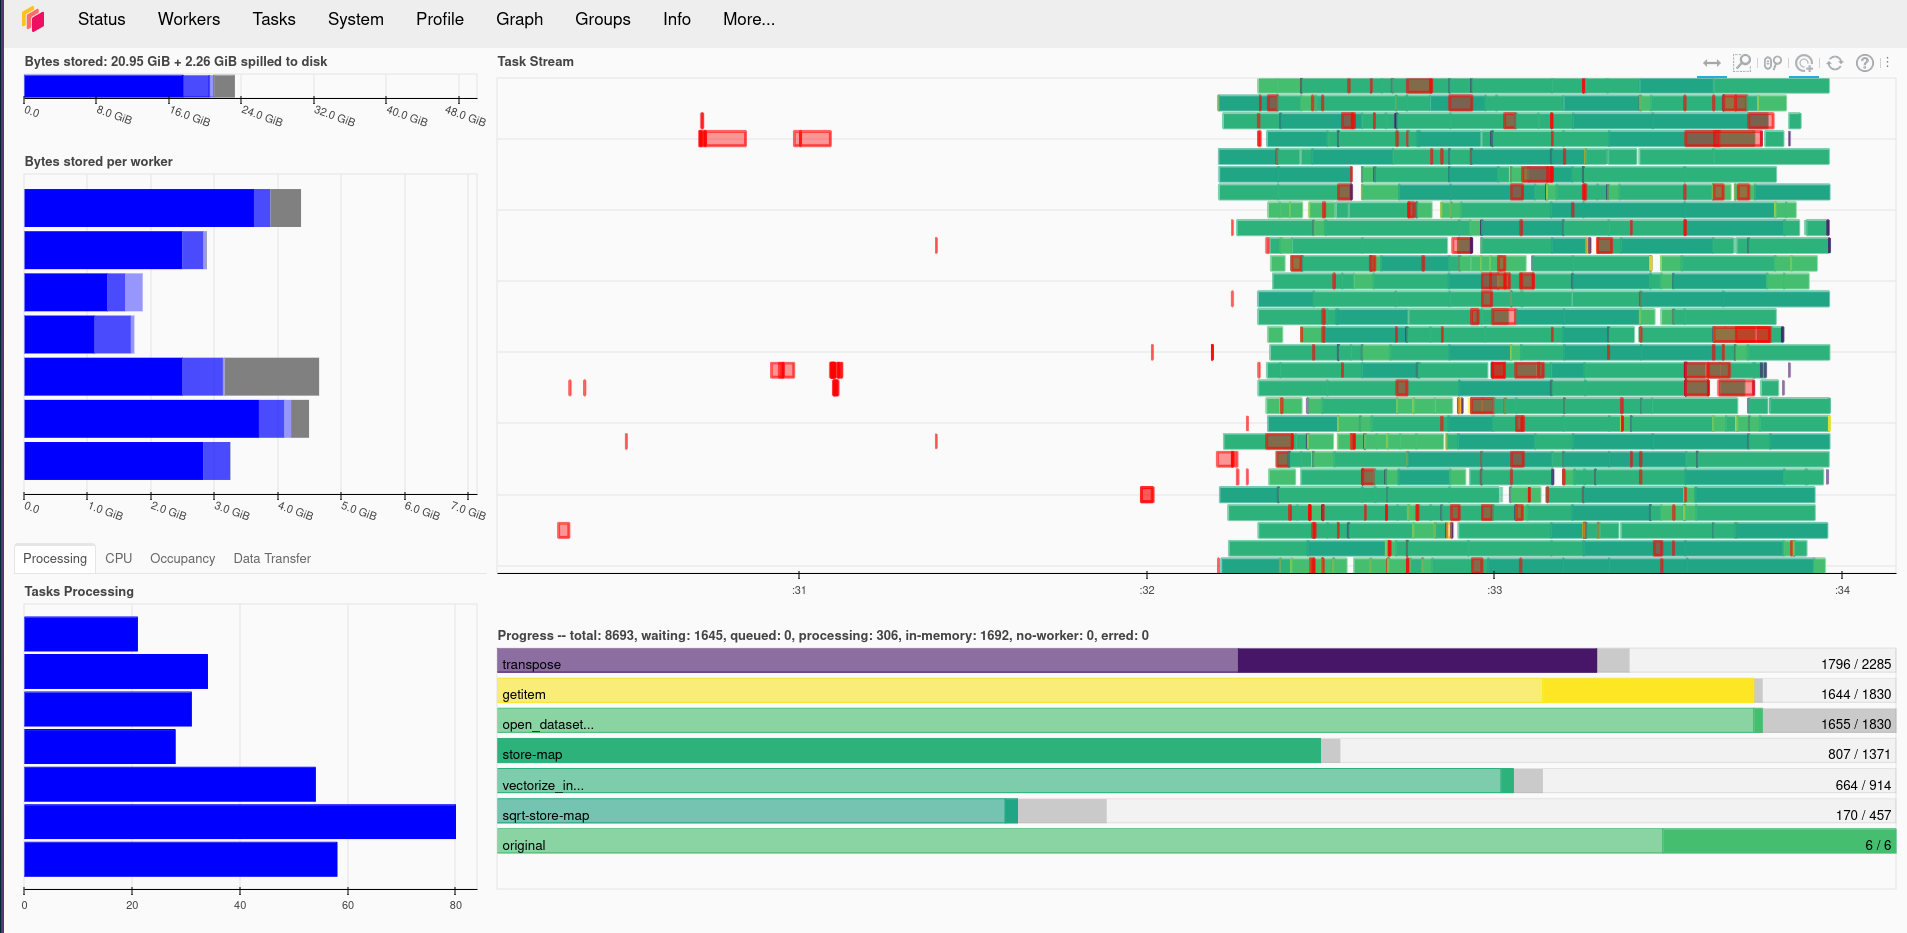
\includegraphics[width=0.95\textwidth]{figures/dask_dashboard_example.png}
  \end{center}
  \caption{Example of the general overview of the dask dashboard used for analyzing the efficiency of the process.}
  \label{fig:dask-dashboard}
\end{figure}


The latter choice is far more important:  
In NetCDF datasets data is often grouped into chunks of a certain, useful size and these chunks can then be compressed to reduce disk memory usage. 
If the chunks are compressed reading anything smaller than a chunk is useless, since the whole chunk needs to be loaded anyway to decompress it. 
Also reading too small chunks reduces the efficiency of dask, since the introduced scheduling overhead per task is too large and becomes overwhelming.
Furthermore, reading too small chunks result in too much worker-to-worker communication, which also results in significantly decreased execution time. 
On the other hand, reading too large chunks results in memory spills\footnote{This refers to a function in dask where overloaded workers save data on disk to prevent the worker from crashing} or workers crashing, which both significantly reduce execution time. 
To find the sweet spot of dask chunk size, dask offers a handy dashboard which visualizes the process of the dask task graph execution (see Figure~\ref{fig:dask-dashboard}). 
Grey areas in the \textit{Bytes stored per worker} section in Figure~\ref{fig:dask-dashboard} show memory spilled to disk, which is an indicator for too large chunk sizes. 
Red sections in the \textit{Task Stream} section refer to worker-to-worker communication, which may be an indicator for too small chunk sizes if they dominate the \textit{Task Stream}. 
So the Task overview given in Figure~\ref{fig:dask-dashboard} indicates a slightly too large chunk size, since too much is spilled to disk. \cite{buckley_choosing_nodate}

The chunk size in the available datasets is $(192, 96, 47, 1)$\footnote{\label{vardims}Referring to $(lon, lat, lev, time)$}, which means one chunk corresponds to one time snapshot of the whole atmosphere.
Following the previous argumentation, the only useful way of changing the chunks are different amounts of time snapshots per chunk.
Using the dask dashboard to evaluate different chunk sizes, the optimal chunk size with minimal spilled memory, worker communication and no crashing workers\footnote{For one of the DKRZ HPC cluster's nodes with 100 GB RAM} was $(192, 96, 47, 128)$\cref{vardims}.  


\textbf{2. Reduction to Area of Interest}

The next step is to cut out the geographical area of interest, which is the northern Atlantic and Europe. 
Following \cite{vietinghoff_visual_2021} and \cite{hurrell_overview_2003}, it was defined as $90^\circ W - 40^\circ E$, $20^\circ - 80^\circ N$.
Unfortunately for this case, the longitude coordinate is saved in the range of $[0,360]^\circ$, so it can't be loaded as one slice. 
Therefor, the longitude coordinates are first transformed to the form $[-180, 180]^\circ$, with negative values being $^\circ W$ and positive values being $^\circ E$. 
Then the area of interest can be cut out without problems and the result can either be used for further calculations (Step 3) or directly saved as a NetCDF file (Step 4). 

\textbf{3. Calculating IVT Field}

The first step to calculate the IVT field is to convert the hybrid sigma pressure levels (see Section \ref{sec:hybridsigma}) to actual pressure values. 
For this Equation \ref{eq:mpige-sigma-hybrid-pressure} is used for calculating a new variable \texttt{plev} containing the pressure values at each gridpoint in each timestep. 
Then NumPy's trapezoidal integration function is used to calculate the zonal (Equation \ref{eq:zonal_ivt}) and meridional (Equation \ref{eq:meridional_ivt}) components of the IVT. 
Similar to related literature \cite{ayantobo_integrated_2022}, a constant value for the gravitational acceleration $g = 9.806~ms^{-2}$ is used in the calculation. 
Using the result of the zonal and meridional components, the norm field $\lVert IVT \rVert$ can be calculated using Equation \ref{eq:ivtnorm}. 



\textbf{4. Saving Results to NetCDF dataset}

The results of these calculations (or the geographical box cutout) are then again saved as NetCDF files, in the far less complex directory structure \texttt{time\_resolution}, \texttt{variable}, \texttt{member} and then the actual file \texttt{timescope.nc}. 
In case of the IVT, both (zonal and merisional) components are saved alongside the Euclidean norm. 


\textbf{5. Generating daily/monthly means}

Since the related literature does not entirely agree regarding the timely resolution of IVT in EOFs (see Table \ref{tab:ivtpatterns-overview}), the six hourly data is reduced to monthly and daily means using CDO.
Monthly IVT is also called stationary moisture transport and dominates the total water vapor transport \cite{zhou_atmospheric_2005}, while the anomalies (departures from monthly mean per daily/subdaily timestep) are transient components.
Both are important parts of total moisture transport, but since a comparison of stationary and transient components is beyond the scope of this thesis, only monthly data will be used for the further analysis. 
The higher resolutions are still saved and can be used in future work. 

% One main goal is to reduce the size, so first the geographic region of interest is cut out, which is the Northern Atlantic (derived from \cite{vietinghoff_visual_2021} and \cite{hurrell_overview_2003}): $-90^\circ W - 40^\circ E$, $20^\circ - 80^\circ N$. 
% For the compared variables (precipitation, surface pressure) the preprocessing is already done, but in case of IVT it still needs to be calculated. 
%
%
% \begin{enumerate}
%   \item Load four different fields for each time period in each member in each scenario: Specific humidity $hus$, eastward horizontal wind $ua$, northward horizontal wind $va$ and surface pressure $ps$. Here the geographical box around the area of interest is cut out: Europe and the North Atlantic (Longitude: $-90 \to 40$, Latitude: $20 \to 80$, based on \cite{vietinghoff_visual_2021})
%   \item For each geographical grid point ($lon$, $lat$) and time step: Calculate the integrals of the product of wind components and specific humidity over the vertical pressure levels $\frac{1}{g}\int_{p_S}^0 hus * ua$ and  $\frac{1}{g}\int_{p_S}^0 hus * va$, with $g$ being the gravitational acceleration ($9.806 \frac{m}{s}$) 
%   \item Save the results for each time period in each member in each scenario in a NetCDF file for the further steps. 
% \end{enumerate}
%
%
%
%
% \textbf{1. Data Loading}
%
% \begin{itemize}
%   \item cutting out geobox
%   \item slow IO $\rightarrow$ started using dask+xarray 
% \end{itemize}
%
% \textbf{2. Vertical Integration}
%
% \begin{itemize}
%   \item calculate hybrid  sigma pressure levels for each gridpoint and timestep to get the x values for integration
%   \item describe my idea of testing the integration
%   
% \end{itemize}
%
\subsection{Problems with Preprocessing}
\label{sec:preprocessing_problems}

The steps described in the section before were just the final attempt. 
The first idea was using Climate Data Operators \cite{schulzweida2024}, a command line tool containing multiple operators for processing climate and similar data. 
The operators consist of common statistical and mathematical functions (mean, add, sum), sampling and data selection tools (select geographical or time limits) and other helpful operators like interpolations and even EOF calculation. 
Although this sounded very promising, it quickly turned out to be very complicated to implement the desired vertical integration in CDO.
The following idea was to implement the IVT calculation in Julia \cite{gao_julia_2020}, using just a NetCDF library \cite{} while the rest was coded from scratch. 
The algorithm was very simple: 

\begin{enumerate}[itemsep=0mm]
  \item Load all datasets into the RAM (as recommended by the NetCDF library itself) and cut out the used geographical limits. This should be feasible since all in all one dataset for one timescope-file accounts for $\sim 12~GB$\footnote{$70~lon * 32~lat * 47~levels * 29220~timesteps * 4~byte \approx 12 GB$}, so the maximum is around $36~GB$, since the surface pressure data is not that large ($\sim 260~MB$)   
  \item Calculate the IVT with trapezoidial integration multithreaded by handling one time\-step by one thread
  \item Write the results (Euclidean norm and the meridional/zonal component)
\end{enumerate}

Although Julia promises high performance, it performed quite poorly on the HPC.
The reason for this is the slow IO on the cluster: While the calculation itself took only $\sim 235~s$ ($\approx 4~min$)\footnote{Refering here and  in the following to one timescope of 20 years in one member}, the loading of the required datasets took around $\sim 3350~s$ ($\approx 55~min$). 
This results in roughly $5 h$ (including saving the data to disk) for one member of ScenarioMIP, which leads to $250~h$ node hours for one scenario. 
Taking into account that it needs to run for historical simulations as well as other scenarios, this was not feasible according to the limited node hours provided\footnote{Also taking into account that the processes may need to run multiple times due to errors}.

To reduce the loading time of the data multiple optimizations were evaluated. 
First, the amount of moved data in memory was minimized by preallocating the needed RAM and writing directly to the preallocated space. 
Furthermore, other NetCDF libraries were tested, but simple loading times were very similar. 
Although this significantly reduced the amount of allocations, the effect on loading time was negligible. 
To actually archive a significant boost in loading time it was tried to load the required datasets (located in different files) in parallel. 
Unfortunately, the used library \cite{barth_ncdatasetsjl_2024} encountered a segmentation fault used in multiple threads, so the alternative libraries NetCDF.jl and HDF5.jl were explored, since the HDF5 standard allows parrallel access to files \cite{folk_overview_2011}. 
Although the parallel access to files using multiple threads (with HDF5.jl) lead to increased speeds in tests, the results did not yield any significant increased efficiency on the cluster itself.
Even splitting up the loading according to the chunking in the files (all data from one timestep is one chunk) and loading each timestep separately in one thread even increased the data loading time quite far.  
The next approach was to split the task up into different processes, each one loading data from one variable. This actually reduced time spent to one third in tests, but testing it on the actual data sizes revealed that the $12~GB$ are too much to be returned from the child processes loading the file to the mother process. 

From here on some other approaches could have been explored, like splitting up different time steps amongst different processes, but the far more suitable method of using xarray and dask has been found and implemented.


\section{EOF Calculation}
